\documentclass[12pt,a4paper]{article}
\usepackage[top=1.5cm, bottom=1.5cm, left=2.0cm, right=1.5cm] {geometry}
\usepackage{amsmath,amssymb,txfonts}
\usepackage{tkz-euclide}
\usepackage{setspace}
\usepackage{lastpage}

\usepackage{tikz,tkz-tab}
%\usepackage[solcolor]{ex_test}
%\usepackage[dethi]{ex_test} % Chỉ hiển thị đề thi
\usepackage[loigiai]{ex_test} % Hiển thị lời giải
%\usepackage[color]{ex_test} % Khoanh các đáp án
\everymath{\displaystyle}

\def\colorEX{\color{purple}}
%\def\colorEX{}%Không tô màu đáp án đúng trong tùy chọn loigiai
\renewtheorem{ex}{\color{violet}Câu}
\renewcommand{\FalseEX}{\stepcounter{dapan}{{\bf \textcolor{blue}{\Alph{dapan}.}}}}
\renewcommand{\TrueEX}{\stepcounter{dapan}{{\bf \textcolor{blue}{\Alph{dapan}.}}}}

%---------- Khai báo viết tắt, in đáp án
\newcommand{\hoac}[1]{ %hệ hoặc
    \left[\begin{aligned}#1\end{aligned}\right.}
\newcommand{\heva}[1]{ %hệ và
    \left\{\begin{aligned}#1\end{aligned}\right.}

%Tiêu đề
\newcommand{\tenso}{iMath}
\newcommand{\tentruong}{Phần mềm Tạo đề ngẫu nhiên}
\newcommand{\tenkythi}{ĐỀ ÔN TẬP}
\newcommand{\tenmonthi}{Môn thi: Toán}
\newcommand{\thoigian}{}
\newcommand{\tieude}[1]{
   \begin{tabular}{cm{3cm}cm{3cm}cm{3cm}}
    {\bf \tenso} & & {\bf \tenkythi} \\
    {\bf \tentruong} & & {\bf \tenmonthi}\\
    && {\bf Thời gian: \bf \thoigian \, phút}\\
    && { \fbox{\bf Mã đề: #1}}
   \end{tabular}\\\\
    
   {Họ tên HS: \dotfill Số báo danh \dotfill}\\
}
\newcommand{\chantrang}[2]{\rfoot{Trang \thepage $-$ Mã đề #2}}
\pagestyle{fancy}
\fancyhf{}
\renewcommand{\headrulewidth}{0pt} 
\renewcommand{\footrulewidth}{0pt}

\begin{document}
%Thiết lập giãn dọng 1.5cm 
%\setlength{\lineskip}{1.5em}
%Nội dung trắc nghiệm bắt đầu ở đây


\tieude{001}
\chantrang{\pageref{LastPage}}{001}
\setcounter{page}{1}
\begin{ex}
	Cho hình chóp ${S.BCDE}$ có đáy là hình vuông tâm ${I}$. Gọi ${P,Q}$ lần lượt là trung điểm của ${SD,SE}$. Giao tuyến của hai mặt phẳng $(IPQ)$ và $(BCDE)$ là 
	\begin{center}
		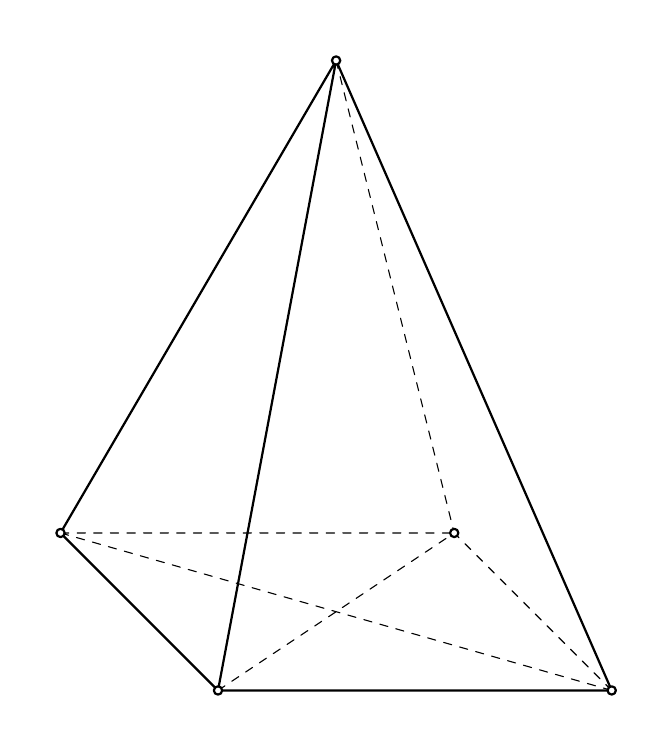
\begin{tikzpicture}[line join=round, line cap=round,thick]
			\coordinate (B) at (0,0);
			\coordinate (C) at (2,-2);
			\coordinate (E) at (5,0);
			\coordinate (D) at ($(C)+(E)-(B)$);
			\coordinate (O) at ($(B)!0.5!(D)$);
			\coordinate (S) at ($(O)+(0,7)$);
			\draw(S)--(B) (S)--(C) (S)--(D) (B)--(C) (C)--(D);
			\draw[dashed,thin](B)--(D) (B)--(E) (D)--(E) (S)--(E) (C)--(E);
			\foreach \i/\g in {S/90,B/180,C/-90,D/-90,E/0}{\draw[fill=white](\i) circle (1.5pt) ($(\i)+(\g:3mm)$) node[scale=1]{};}
		\end{tikzpicture}
		
	\end{center}
	\choice
	{ đường thẳng qua ${S}$ và song song với ${CD}$ }
	{ \True đường thẳng qua ${I}$ và song song với ${DE}$ }
	{ đường thẳng qua ${S}$ và song song với ${BC}$ }
	{ đường thẳng qua ${S}$ và song song với ${BE}$ }
	\loigiai{\begin{center}
			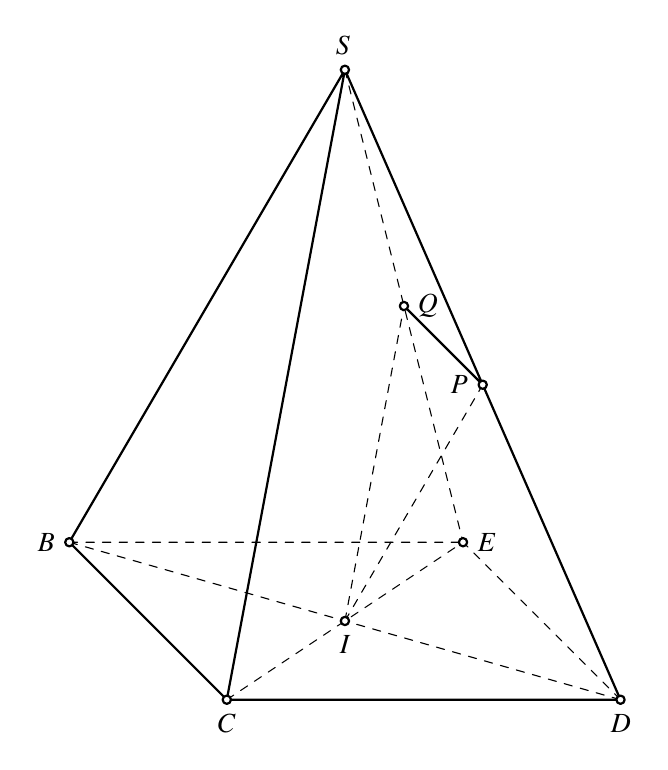
\begin{tikzpicture}[line join=round, line cap=round,thick]
				\coordinate (B) at (0,0);
				\coordinate (C) at (2,-2);
				\coordinate (E) at (5,0);
				\coordinate (D) at ($(C)+(E)-(B)$);
				\coordinate (I) at ($(B)!0.5!(D)$);
				\coordinate (S) at ($(I)+(0,7)$);
				\coordinate (P) at ($(S)!0.5!(D)$);
				\coordinate (Q) at ($(S)!0.5!(E)$);
				\draw(S)--(B) (S)--(C) (S)--(D) (B)--(C) (C)--(D) (P)--(Q);
				\draw[dashed,thin](B)--(D) (B)--(E) (D)--(E) (S)--(E) (C)--(E);
				\draw[dashed,thin](I)--(P) (I)--(Q) ;
				\foreach \i/\g in {S/90,B/180,C/-90,D/-90,E/0,I/-90,P/180,Q/0}{\draw[fill=white](\i) circle (1.5pt) ($(\i)+(\g:3mm)$) node[scale=1]{$\i$};}
			\end{tikzpicture}
			
		\end{center}
		$\left\{ \begin{array}{l} 
			PQ\subset (IPQ) \\ 
			DE\subset (BCDE)\\ 
			PQ // DE 
		\end{array} \right.$$\Rightarrow (IPQ) \cap (BCDE)=Ix // DE //PQ //BC$. 
}\end{ex}






\newpage 



\end{document}